\section{Bancos de dados colunares} \label{colunar}
A idéia por traz dos bancos de dados colunares não é nova. Uma das primeiras propostas de organizar os dados de um banco de dados por colunas, em vez da tradicional representação por linhas dos bancos de dados relacionais, apareceu em 1969 \cite{Estabrook1969327}. De forma resumida, enquanto um banco de dados relacional armazena cada registro (tupla) em um espaço contínuo do disco (ou memória), os bancos de dados colunares armazenam cada coluna em espaços contínuos. Para isso, cada coluna de uma tabela (ou relação), é dividia em um índice com os valores distintos ordenados e um vetor com a codificação dos valores de cada tupla na mesma sequência em que aparecem na tabela. A Figura \ref{fig:tabular} mostra a representação tradicional de uma tabela num banco de dados relacional e a Figura \ref{fig:colunar} mostra como a primeira coluna da relação é organizada em um banco de dados colunar.

\begin{figure}
	\centering
	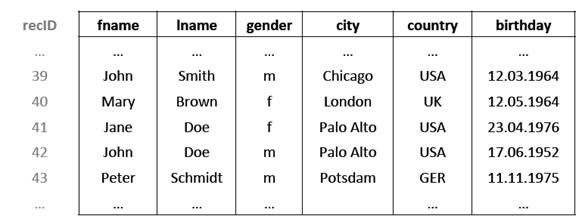
\includegraphics[width=\linewidth]{./colunar_repr_tabela.png}
	\caption{Representação de uma tabela em um banco de dados relacional.}
	\label{fig:tabular}
\end{figure}

\begin{figure}
	\centering
	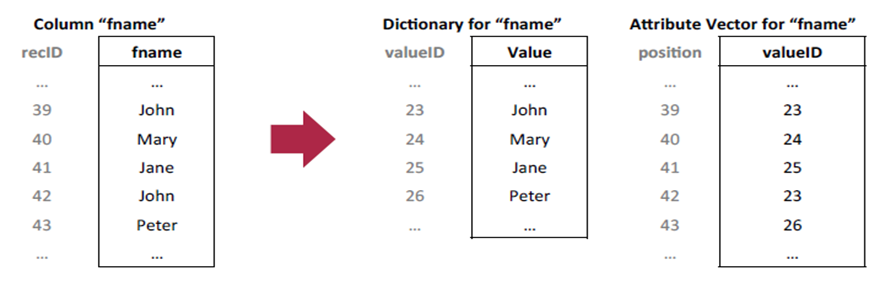
\includegraphics[width=\linewidth]{./colunar_repr_coluna.png}
	\caption{Organização da coluna fname em um banco de dados colunar.}
	\label{fig:colunar}
\end{figure}

A grande vantagem da representação colunar é a compressão de dados, que ocorre, principalmente, pela codificação com um numero mínimo de bits dos valores de cada registro, baseada no dicionário. Com os dados comprimidos, menos Bytes trafegam entre o disco e a memória principal, tornando operações de consulta e agregação mais rápidas.

Para explicar melhor, imaginemos que a coluna \textbf{fname} tenha 100 caracteres representados por 1 Byte cada. Imaginemos também que a tabela em questão trata-se da lista de todos os cidadãos brasileiros, ou seja, teremos 200 milhões de registros. Logo, o espaço de armazenamento no modelo tradicional é de $ 200*10^6 * 100 Bytes \cong 18,62 GBytes  $. No armazenamento em formato de colunas, os dados são armazenados em um dicionário que contém uma entrada para cada valor distinto. Imaginemos que há 10 mil primeiro nomes distintos no Brasil. Com isso, para o dicionário, precisamos de $ 10*10^3 * 100 Bytes \cong 1 MBytes  $. Já o vetor de valores conterá os 200 milhões de registros, mas codificados pela quantidade mínima de bits necessários para se codificar os 10 mil valores distintos $ log_2 10000 \cong 13,2  $, ou seja, 14 bits. Nesse caso, o vetor de valores terá $ 200*10^6 * 14 bits \cong 2,6 GBytes  $. Nesse simples exemplo, podemos ver um fator de compressão de $ 18,62 / (0,001 + 2,6) \cong 7,2 $ vezes.

A recuperação de um determinado registro (tupla) passa por um acesso direto à posição dele em cada uma dos vetores de valor das colunas da tabela e mais um acesso em cada dicionário para traduzir a codificação no valor original.

O grande problema nessa representação são operações de remoção e inserção, que usualmente causam uma reorganização do dicionário e consequentemente uma reorganização de todos os dados da coluna cujo dicionário foi reordenado. Por isso, o uso desse tipo de tecnologia deve ser preferível em conjuntos de dados cuja operação predominante seja de consulta. Plattner \cite{plattner2009common} alega que os bancos de dados corporativos possuem uma carga predominantemente de consulta e com isso, pode-se unificar os repositórios OLTP e OLAP na mesma estrutura. 

Os sistemas modernos que utilizam a representação colunar lançam mão de diversas estratégias para minimizar esses efeitos de reorganização dos dicionários. O SAP HANA, por exemplo, divide os dados em principal e diferencial \cite{plattner2012memory}. Novos registros e atualizações de valores são incluídos no conjunto diferencial, que é mantido em tamanho pequeno. As operações de consulta juntam os dados do conjunto principal com o conjunto diferencial. Embora a busca no conjunto diferencial seja ineficiente, ela é realizada sobre um conjunto pequeno de dados. De tempos em tempos, os conjuntos são mesclados resultando em um novo conjunto principal e um conjunto diferencial praticamente vazio, que conterá apenas as operações realizadas durante a operação de mesclagem.

Atualmente, os principais fornecedores de bancos de dados relacionais também fornecem soluções de armazenamento colunar, como Microsoft, Oracle, IBM, SAP e outros.  




